\documentclass[aspectratio=169,11pt]{beamer}

\usetheme{SimplePlus}

\usepackage{amsmath}
\usepackage{amssymb}
\usepackage{booktabs}
\usepackage{graphicx}
\usepackage{array}
\usepackage{tikz}

\title{S181M116 Derivatives and Alternative Investments}
\subtitle{Lecture 4: Options, Put-Call Parity, and Binomial Trees}
\author{Swapnil Singh}
\institute{Lietuvos Bankas and Kaunas University of Technology}
\date{}

\newcommand{\St}{S_T}
\newcommand{\Szero}{S_0}
\newcommand{\K}{K}
\newcommand{\T}{T}
\newcommand{\dt}{\Delta t}
\newcommand{\erdt}{e^{-r\Delta t}}
\newcommand{\erT}{e^{-rT}}
\newcommand{\PV}{\mathrm{PV}}
\newcommand{\Div}{D}

\AtBeginSection[]{
    \begin{frame}[plain,noframenumbering]
        \vfill
        \begin{center}
            {\usebeamerfont{subtitle}\usebeamercolor[fg]{structure}Section \thesection\par}
            \vspace{0.5em}
            {\usebeamerfont{title}\usebeamercolor[fg]{titlelike}\insertsectionhead\par}
        \end{center}

        \vspace{1.2em}
        \begin{center}
            \begin{minipage}{0.72\textwidth}
                \tableofcontents[currentsection,hideothersubsections]
            \end{minipage}
        \end{center}
        \vfill
    \end{frame}
}

\begin{document}

\begin{frame}
    \titlepage
\end{frame}

\begin{frame}{Today}
    \begin{enumerate}
        \item What options are and how they differ from forwards and futures.
        \item How calls, puts, long positions, and short positions pay off.
        \item How option contracts are specified, traded, margined, cleared, and customized.
        \item Which inputs move option prices.
        \item How no-arbitrage gives option bounds and put-call parity.
        \item When early exercise matters for American options.
        \item How binomial trees price European and American options.
        \item How delta connects option pricing and hedging.
    \end{enumerate}
\end{frame}

\begin{frame}{Core Message}
    \begin{block}{Options are asymmetric contracts}
        \begin{itemize}
            \item The \textbf{holder} has a right, not an obligation.
            \item The \textbf{writer} receives the premium, but accepts a contingent obligation.
            \item The premium is paid up front because the payoff is one-sided.
        \end{itemize}
    \end{block}

    \vspace{0.6em}
    \begin{alertblock}{Pricing lesson}
        We do not price an option by discounting an expected payoff at an arbitrary risky rate.
        We price it by no-arbitrage relative to the underlying asset and the risk-free asset.
    \end{alertblock}
\end{frame}

\section{Option Contracts and Markets}

\begin{frame}{Forwards versus Options}
    \begin{columns}[T]
        \begin{column}{0.48\textwidth}
            \begin{block}{Forward or futures contract}
                \begin{itemize}
                    \item Both parties commit to a future transaction.
                    \item Long and short payoffs are symmetric.
                    \item Initial contract value is often close to zero.
                    \item Margin may be required, but no option premium is paid.
                \end{itemize}
            \end{block}
        \end{column}
        \begin{column}{0.48\textwidth}
            \begin{block}{Option contract}
                \begin{itemize}
                    \item Holder chooses whether to exercise.
                    \item Writer must perform if assigned.
                    \item Payoff is asymmetric.
                    \item Holder pays an option premium up front.
                \end{itemize}
            \end{block}
        \end{column}
    \end{columns}

    \vspace{0.5em}
    Options are valuable because the holder can keep favorable states and discard unfavorable states.
\end{frame}

\begin{frame}{Calls and Puts}
    \begin{columns}[T]
        \begin{column}{0.48\textwidth}
            \begin{block}{Call option}
                Right to \textbf{buy} the underlying asset at strike \(K\).
                \[
                    \text{payoff}=\max(S_T-K,0).
                \]
                The call holder benefits from higher underlying prices.
            \end{block}
        \end{column}
        \begin{column}{0.48\textwidth}
            \begin{block}{Put option}
                Right to \textbf{sell} the underlying asset at strike \(K\).
                \[
                    \text{payoff}=\max(K-S_T,0).
                \]
                The put holder benefits from lower underlying prices.
            \end{block}
        \end{column}
    \end{columns}

    \vspace{0.6em}
    The strike price is the exercise price. The expiration date is the last date relevant for exercise.
\end{frame}

\begin{frame}{Intuition Example: Insurance}
    Think of a put option as price insurance.

    \begin{exampleblock}{Investor owns a stock at 100}
        The investor buys a three-month put with strike 95.
        \begin{itemize}
            \item If the stock falls to 70, the put allows sale at 95.
            \item If the stock rises to 120, the investor ignores the put and keeps the upside.
            \item The premium is the cost of this protection.
        \end{itemize}
    \end{exampleblock}

    \begin{block}{Teaching point}
        The put does not prevent the stock price from falling.
        It changes the investor's payoff after the fall.
    \end{block}
\end{frame}

\begin{frame}{Intuition Example: Reservation Price}
    Think of a call option as locking in a maximum purchase price.

    \begin{exampleblock}{Firm may need copper in three months}
        The firm buys a call with strike 9,000 per ton.
        \begin{itemize}
            \item If copper rises to 10,500, the call lets the firm buy at 9,000.
            \item If copper falls to 8,000, the firm buys in the market and lets the call expire.
            \item The premium pays for flexibility.
        \end{itemize}
    \end{exampleblock}

    \begin{alertblock}{Comparison with a forward}
        A forward would lock in the purchase price both when copper rises and when copper falls.
    \end{alertblock}
\end{frame}

\begin{frame}{European and American Exercise}
    \begin{block}{European option}
        Can be exercised only at maturity.
    \end{block}

    \begin{block}{American option}
        Can be exercised at any time up to and including maturity.
    \end{block}

    \vspace{0.4em}
    These names describe exercise style, not geography.

    \begin{alertblock}{Value implication}
        American exercise cannot make the holder worse off:
        \[
            C\geq c,
            \qquad
            P\geq p.
        \]
        Here \(C,P\) are American prices and \(c,p\) are European prices.
    \end{alertblock}
\end{frame}

\begin{frame}{Payoff versus Profit}
    \begin{block}{Payoff}
        Cash value received at maturity before subtracting the premium.
    \end{block}

    \begin{block}{Profit}
        Payoff minus the initial premium, usually ignoring time value of money in diagrams.
    \end{block}

    \begin{exampleblock}{Call with \(K=100\) and premium \(5\)}
        If \(S_T=102\), the holder exercises:
        \[
            \text{payoff}=2,
            \qquad
            \text{profit}=2-5=-3.
        \]
        Exercising still reduces the loss relative to letting the option expire worthless.
    \end{exampleblock}
\end{frame}

\begin{frame}{Long Call Payoff}
    \begin{columns}[T]
        \begin{column}{0.46\textwidth}
            \[
                \text{payoff}=\max(S_T-K,0)
            \]
            \begin{itemize}
                \item Limited downside: premium paid.
                \item Potentially unlimited upside for a stock.
                \item Break-even at \(S_T=K+\text{premium}\).
            \end{itemize}
        \end{column}
        \begin{column}{0.50\textwidth}
            \begin{center}
            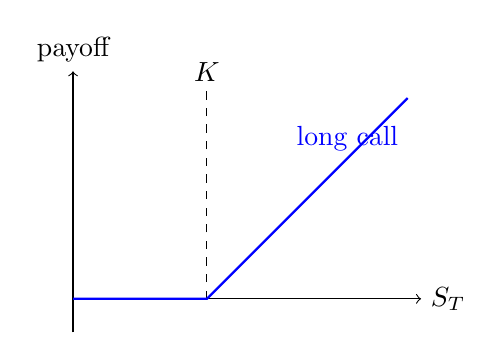
\begin{tikzpicture}[scale=0.85]
                \draw[->] (0,0) -- (5.2,0) node[right] {\(S_T\)};
                \draw[->] (0,-0.5) -- (0,3.4) node[above] {payoff};
                \draw[dashed] (2,0) -- (2,3.1) node[above] {\(K\)};
                \draw[thick,blue] (0,0) -- (2,0) -- (5,3);
                \node[blue] at (4.1,2.4) {long call};
            \end{tikzpicture}
            \end{center}
        \end{column}
    \end{columns}
\end{frame}

\begin{frame}{Long Put Payoff}
    \begin{columns}[T]
        \begin{column}{0.46\textwidth}
            \[
                \text{payoff}=\max(K-S_T,0)
            \]
            \begin{itemize}
                \item Limited downside: premium paid.
                \item Payoff rises as the asset falls.
                \item Break-even at \(S_T=K-\text{premium}\).
            \end{itemize}
        \end{column}
        \begin{column}{0.50\textwidth}
            \begin{center}
            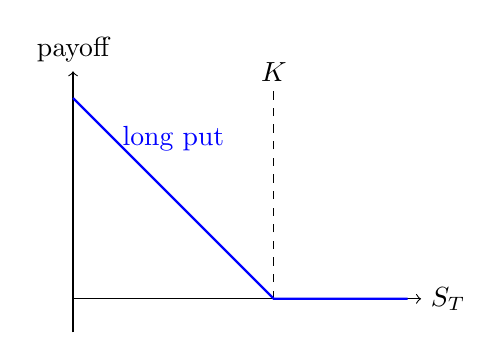
\begin{tikzpicture}[scale=0.85]
                \draw[->] (0,0) -- (5.2,0) node[right] {\(S_T\)};
                \draw[->] (0,-0.5) -- (0,3.4) node[above] {payoff};
                \draw[dashed] (3,0) -- (3,3.1) node[above] {\(K\)};
                \draw[thick,blue] (0,3) -- (3,0) -- (5,0);
                \node[blue] at (1.5,2.4) {long put};
            \end{tikzpicture}
            \end{center}
        \end{column}
    \end{columns}
\end{frame}

\begin{frame}{The Four Basic Positions}
    \small
    \begin{center}
    \begin{tabular}{lll}
        \toprule
        Position & Payoff at maturity & Risk profile \\
        \midrule
        Long call & \(\max(S_T-K,0)\) & Pays premium; benefits from upside \\
        Short call & \(-\max(S_T-K,0)\) & Receives premium; loses on upside \\
        Long put & \(\max(K-S_T,0)\) & Pays premium; benefits from downside \\
        Short put & \(-\max(K-S_T,0)\) & Receives premium; loses on downside \\
        \bottomrule
    \end{tabular}
    \end{center}

    \vspace{0.8em}
    \begin{alertblock}{Writer risk}
        Short option positions receive cash today but create possible future liabilities.
        This is why option writers face margin requirements.
    \end{alertblock}
\end{frame}

\begin{frame}{Example: Covered Call versus Naked Call}
    \begin{columns}[T]
        \begin{column}{0.48\textwidth}
            \begin{block}{Covered call}
                Investor owns 100 shares and writes one call.
                \begin{itemize}
                    \item Premium provides income.
                    \item Upside above the strike is given away.
                    \item If assigned, the investor delivers shares already owned.
                \end{itemize}
            \end{block}
        \end{column}
        \begin{column}{0.48\textwidth}
            \begin{alertblock}{Naked short call}
                Investor writes the call without owning shares.
                \begin{itemize}
                    \item Premium is received up front.
                    \item If the stock rises sharply, losses can be very large.
                    \item The writer must buy shares at the market price to deliver at \(K\).
                \end{itemize}
            \end{alertblock}
        \end{column}
    \end{columns}
\end{frame}

\begin{frame}{Moneyness}
    \begin{center}
    \begin{tabular}{lll}
        \toprule
        & Call & Put \\
        \midrule
        In the money & \(S>K\) & \(S<K\) \\
        At the money & \(S=K\) & \(S=K\) \\
        Out of the money & \(S<K\) & \(S>K\) \\
        \bottomrule
    \end{tabular}
    \end{center}

    \begin{block}{Intrinsic value}
        \[
            \text{Call intrinsic value}=\max(S-K,0),
            \qquad
            \text{Put intrinsic value}=\max(K-S,0).
        \]
    \end{block}

    \begin{block}{Time value}
        \[
            \text{Time value}=\text{option price}-\text{intrinsic value}.
        \]
    \end{block}
\end{frame}

\begin{frame}{Example: Reading an Option Quote}
    A stock trades at 48. A quoted option is:
    \[
        \text{XYZ 50 call, two months, price } 2.40.
    \]

    \begin{itemize}
        \item It is a call, so it gives the right to buy.
        \item The strike is 50.
        \item It is out of the money because \(48<50\).
        \item Intrinsic value is \(\max(48-50,0)=0\).
        \item The full 2.40 price is time value.
        \item One standard contract costs \(2.40\times 100=240\).
    \end{itemize}

    \begin{block}{Question for students}
        What stock price at expiration is needed to break even, ignoring interest?
    \end{block}
\end{frame}

\begin{frame}{Stock Option Contract Terms}
    \begin{itemize}
        \item A standard U.S. exchange-traded stock option contract usually covers 100 shares.
        \item A quoted price is typically per share.
        \item A quote of \(4.20\) means a premium of \(4.20\times 100=420\) for one contract.
        \item Exchanges specify expiration dates, strikes, exercise style, contract size, and adjustment rules.
        \item Weekly options and longer-term LEAPS add maturity choices beyond standard monthly cycles.
    \end{itemize}

    \begin{block}{Class versus series}
        \textbf{Option class:} all calls or all puts on the same underlying.

        \textbf{Option series:} same type, same underlying, same strike, and same expiration.
    \end{block}
\end{frame}

\begin{frame}{Dividends, Splits, and Adjustments}
    \begin{block}{Cash dividends}
        Ordinary cash dividends usually do not mechanically adjust exchange-traded stock option terms.
        Expected dividends enter option prices because they affect the stock price path.
    \end{block}

    \begin{block}{Stock splits and stock dividends}
        Contract terms are adjusted to preserve economic exposure.
    \end{block}

    \begin{exampleblock}{Two-for-one split}
        A call on 100 shares with strike 30 becomes a call on 200 shares with strike 15.
        \[
            100\times 30=200\times 15=3000.
        \]
    \end{exampleblock}
\end{frame}

\begin{frame}{Trading, Clearing, and Margin}
    \begin{columns}[T]
        \begin{column}{0.48\textwidth}
            \begin{block}{Market makers}
                Quote bid and ask prices, provide liquidity, earn bid-ask spreads, and hedge inventory risk.
            \end{block}

            \begin{block}{Offsetting orders}
                Most positions are closed by trading the same option series in the opposite direction.
            \end{block}
        \end{column}
        \begin{column}{0.48\textwidth}
            \begin{block}{Margin}
                Buyers pay the premium and have no further obligation.
                Writers have contingent obligations and must post margin.
            \end{block}

            \begin{block}{OCC}
                The Options Clearing Corporation records positions, handles exercise, and guarantees performance.
            \end{block}
        \end{column}
    \end{columns}
\end{frame}

\begin{frame}{Exchange-Traded and OTC Options}
    \begin{columns}[T]
        \begin{column}{0.48\textwidth}
            \begin{block}{Exchange-traded}
                \begin{itemize}
                    \item Standardized contract terms.
                    \item Central clearing.
                    \item Transparent listed markets.
                    \item Lower counterparty risk.
                \end{itemize}
            \end{block}
        \end{column}
        \begin{column}{0.48\textwidth}
            \begin{block}{Over the counter}
                \begin{itemize}
                    \item Customized strikes, maturities, payoffs, and settlement.
                    \item Useful for institutional hedging.
                    \item Exposes parties to credit, collateral, model, and liquidity risk.
                \end{itemize}
            \end{block}
        \end{column}
    \end{columns}

    \vspace{0.5em}
    Related contracts include warrants, employee stock options, and convertible bonds.
\end{frame}

\section{Option Price Restrictions}

\begin{frame}{Six Inputs to a Stock Option Price}
    \begin{enumerate}
        \item Current stock price \(S_0\).
        \item Strike price \(K\).
        \item Time to expiration \(T\).
        \item Volatility \(\sigma\).
        \item Risk-free interest rate \(r\).
        \item Expected dividends during the option's life.
    \end{enumerate}

    \vspace{0.5em}
    \begin{center}
    \begin{tabular}{lll}
        \toprule
        Increase in input & Call value & Put value \\
        \midrule
        \(S_0\) & Increases & Decreases \\
        \(K\) & Decreases & Increases \\
        \(\sigma\) & Increases & Increases \\
        \(r\) & Usually increases & Usually decreases \\
        Expected dividends & Decreases & Increases \\
        \bottomrule
    \end{tabular}
    \end{center}
\end{frame}

\begin{frame}{Why Volatility Raises Both Calls and Puts}
    \begin{block}{The underlying owner faces both sides}
        A stock investor gains from upside and loses from downside.
    \end{block}

    \begin{block}{The option holder keeps only one side}
        \begin{itemize}
            \item A call keeps upside above \(K\) and discards downside below \(K\).
            \item A put keeps downside below \(K\) and discards upside above \(K\).
        \end{itemize}
    \end{block}

    \begin{alertblock}{Convex payoff}
        Higher uncertainty makes convex payoffs more valuable, holding the current underlying price fixed.
    \end{alertblock}
\end{frame}

\begin{frame}{Intuition Example: Same Average, Different Volatility}
    Consider a call with strike 100.

    \begin{columns}[T]
        \begin{column}{0.48\textwidth}
            \begin{block}{Low-volatility world}
                Stock ends at:
                \[
                    98 \quad \text{or} \quad 102.
                \]
                Call payoff:
                \[
                    0 \quad \text{or} \quad 2.
                \]
            \end{block}
        \end{column}
        \begin{column}{0.48\textwidth}
            \begin{block}{High-volatility world}
                Stock ends at:
                \[
                    80 \quad \text{or} \quad 120.
                \]
                Call payoff:
                \[
                    0 \quad \text{or} \quad 20.
                \]
            \end{block}
        \end{column}
    \end{columns}

    \vspace{0.5em}
    Both worlds can have the same average stock price, but the call is much more valuable in the high-volatility world.
\end{frame}

\begin{frame}{Upper Bounds}
    \begin{block}{Calls}
        A call cannot be worth more than the stock:
        \[
            c\leq S_0,
            \qquad
            C\leq S_0.
        \]
    \end{block}

    \begin{block}{Puts}
        A put cannot be worth more than the strike:
        \[
            p\leq K,
            \qquad
            P\leq K.
        \]
        For a European put, a sharper bound is
        \[
            p\leq K e^{-rT}.
        \]
    \end{block}
\end{frame}

\begin{frame}{Lower Bound for a European Call}
    For a non-dividend-paying stock:
    \[
        c\geq \max(S_0-Ke^{-rT},0).
    \]

    \begin{block}{Dominance argument}
        Compare:
        \begin{itemize}
            \item Portfolio A: one European call plus cash \(Ke^{-rT}\);
            \item Portfolio B: one share.
        \end{itemize}
        At maturity, Portfolio A is worth at least the stock in every state.
    \end{block}

    \begin{exampleblock}{Example}
        If \(S_0=20\), \(K=18\), \(r=10\%\), \(T=1\):
        \[
            c\geq 20-18e^{-0.10}=3.71.
        \]
    \end{exampleblock}
\end{frame}

\begin{frame}{Lower Bound for a European Put}
    For a non-dividend-paying stock:
    \[
        p\geq \max(Ke^{-rT}-S_0,0).
    \]

    \begin{block}{Dominance argument}
        Compare:
        \begin{itemize}
            \item Portfolio A: one European put plus one share;
            \item Portfolio B: cash \(Ke^{-rT}\).
        \end{itemize}
        At maturity, Portfolio A is worth at least \(K\) in every state.
    \end{block}

    \begin{exampleblock}{Example}
        If \(S_0=37\), \(K=40\), \(r=5\%\), \(T=0.5\):
        \[
            p\geq 40e^{-0.025}-37=2.01.
        \]
    \end{exampleblock}
\end{frame}

\begin{frame}{Put-Call Parity}
    For European options on a non-dividend-paying stock:
    \[
        c+Ke^{-rT}=p+S_0.
    \]

    \begin{columns}[T]
        \begin{column}{0.48\textwidth}
            \begin{block}{Fiduciary call}
                \[
                    \text{call}+\text{cash }Ke^{-rT}
                \]
                Pays \(\max(S_T,K)\) at maturity.
            \end{block}
        \end{column}
        \begin{column}{0.48\textwidth}
            \begin{block}{Protective put}
                \[
                    \text{put}+\text{stock}
                \]
                Pays \(\max(S_T,K)\) at maturity.
            \end{block}
        \end{column}
    \end{columns}

    \vspace{0.5em}
    Identical future payoffs must have identical current values.
\end{frame}

\begin{frame}{Parity State-by-State}
    \begin{center}
    \begin{tabular}{llll}
        \toprule
        State at \(T\) & Call + cash & Put + stock & Common payoff \\
        \midrule
        \(S_T>K\) & \(S_T-K+K\) & \(0+S_T\) & \(S_T\) \\
        \(S_T\leq K\) & \(0+K\) & \(K-S_T+S_T\) & \(K\) \\
        \bottomrule
    \end{tabular}
    \end{center}

    \vspace{0.8em}
    Therefore:
    \[
        c-p=S_0-Ke^{-rT}.
    \]

    \begin{alertblock}{Interpretation}
        The call-put price difference equals the forward-like value of buying the stock and financing the strike.
    \end{alertblock}
\end{frame}

\begin{frame}{Intuition Example: Two Ways to Guarantee a Floor}
    Suppose \(K=100\). There are two ways to guarantee that the final portfolio is worth at least 100.

    \begin{columns}[T]
        \begin{column}{0.48\textwidth}
            \begin{block}{Protective put}
                Buy the stock and buy a put.
                \[
                    S_T+\max(100-S_T,0)
                    =
                    \max(S_T,100).
                \]
            \end{block}
        \end{column}
        \begin{column}{0.48\textwidth}
            \begin{block}{Fiduciary call}
                Buy a call and lend the present value of 100.
                \[
                    \max(S_T-100,0)+100
                    =
                    \max(S_T,100).
                \]
            \end{block}
        \end{column}
    \end{columns}

    \begin{alertblock}{Parity intuition}
        If two strategies deliver the same insured payoff, they must cost the same today.
    \end{alertblock}
\end{frame}

\begin{frame}{Parity Example}
    Suppose
    \[
        S_0=31,
        \qquad
        K=30,
        \qquad
        r=6\%,
        \qquad
        T=0.25,
        \qquad
        c=3.
    \]

    Put-call parity implies
    \[
        p=c+Ke^{-rT}-S_0.
    \]

    Hence
    \[
        p=3+30e^{-0.06(0.25)}-31
        \approx 1.55.
    \]
\end{frame}

\begin{frame}{Parity Arbitrage}
    If
    \[
        c+Ke^{-rT}>p+S_0,
    \]
    the fiduciary call is expensive. Sell it and buy the protective put:
    \[
        \text{short call, borrow }Ke^{-rT},\text{ buy put, buy stock}.
    \]

    \vspace{0.6em}
    If
    \[
        c+Ke^{-rT}<p+S_0,
    \]
    the protective put is expensive. Buy the fiduciary call and sell the protective put:
    \[
        \text{buy call, lend }Ke^{-rT},\text{ short put, short stock}.
    \]

    \begin{alertblock}{Reality check}
        Transaction costs, bid-ask spreads, short-sale constraints, and funding spreads determine whether the arbitrage is implementable.
    \end{alertblock}
\end{frame}

\begin{frame}{Dividends and Put-Call Parity}
    Let \(D\) be the present value of known cash dividends during the option's life.

    \begin{block}{Dividend-adjusted parity}
        \[
            c+D+Ke^{-rT}=p+S_0.
        \]
        Equivalently:
        \[
            c-p=S_0-D-Ke^{-rT}.
        \]
    \end{block}

    \begin{block}{Lower bounds}
        \[
            c\geq \max(S_0-D-Ke^{-rT},0),
        \]
        \[
            p\geq \max(Ke^{-rT}+D-S_0,0).
        \]
    \end{block}
\end{frame}

\begin{frame}{American Options and Parity Inequalities}
    Exact European put-call parity generally does not hold for American options because early exercise can matter.

    \begin{block}{Non-dividend-paying stock}
        \[
            S_0-K\leq C-P\leq S_0-Ke^{-rT}.
        \]
    \end{block}

    \begin{itemize}
        \item American calls on non-dividend-paying stocks have no early-exercise premium.
        \item American puts may have an early-exercise premium.
        \item Therefore American parity becomes an inequality, not an equality.
    \end{itemize}
\end{frame}

\section{Early Exercise}

\begin{frame}{American Calls Without Dividends}
    \begin{alertblock}{Result}
        It is never optimal to exercise an American call early on a non-dividend-paying stock.
    \end{alertblock}

    Exercising early gives up:
    \begin{enumerate}
        \item the time value of the option;
        \item the ability to delay paying the strike \(K\);
        \item downside protection if the stock later falls.
    \end{enumerate}

    \vspace{0.6em}
    Therefore:
    \[
        C=c
    \]
    for an otherwise identical non-dividend-paying stock call.
\end{frame}

\begin{frame}{Example: Why Not Exercise a Call Early?}
    You hold an American call on a non-dividend-paying stock:
    \[
        S=120,\qquad K=100,\qquad \text{six months remaining.}
    \]

    Exercising now gives intrinsic value:
    \[
        120-100=20.
    \]

    But selling the call is usually better because the call price includes:
    \begin{itemize}
        \item intrinsic value;
        \item remaining time value;
        \item the benefit of not paying \(K\) until later.
    \end{itemize}

    \begin{alertblock}{Classroom takeaway}
        If you want to exit, sell the call. Do not throw away time value by exercising early.
    \end{alertblock}
\end{frame}

\begin{frame}{American Puts Without Dividends}
    \begin{alertblock}{Result}
        Early exercise of an American put can be optimal.
    \end{alertblock}

    \begin{itemize}
        \item A deep-in-the-money put allows the holder to sell the stock for \(K\).
        \item If the stock price is very low, immediate exercise produces cash early.
        \item Receiving \(K\) early is valuable when interest rates are positive.
    \end{itemize}

    \vspace{0.6em}
    The American put must be worth at least intrinsic value:
    \[
        P\geq \max(K-S_0,0).
    \]
\end{frame}

\begin{frame}{Dividends and Early Exercise}
    \begin{block}{Calls}
        Dividends can make early exercise optimal.
        A call holder does not receive dividends unless the option is exercised and converted into stock.
    \end{block}

    \begin{block}{Puts}
        Dividends reduce the stock price when the stock goes ex-dividend, which can make waiting more attractive for puts.
    \end{block}

    \begin{alertblock}{Practical rule}
        Early exercise depends on moneyness, interest rates, dividend timing, dividend size, and remaining time value.
    \end{alertblock}
\end{frame}

\section{Binomial Trees}

\begin{frame}{One-Step Binomial Setup}
    Over one period, the stock moves from \(S_0\) to one of two values:
    \[
        S_u=S_0u,
        \qquad
        S_d=S_0d,
        \qquad
        u>1,\quad d<1.
    \]

    \begin{center}
    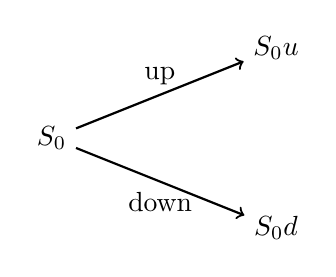
\begin{tikzpicture}[scale=0.95]
        \node (s0) at (0,0) {\(S_0\)};
        \node (su) at (3,1.2) {\(S_0u\)};
        \node (sd) at (3,-1.2) {\(S_0d\)};
        \draw[->,thick] (s0) -- (su) node[midway,above] {up};
        \draw[->,thick] (s0) -- (sd) node[midway,below] {down};
    \end{tikzpicture}
    \end{center}

    Let the option values at the two final nodes be \(f_u\) and \(f_d\).
\end{frame}

\begin{frame}{Intuition Example: A Tiny Replication Problem}
    Suppose a stock is 20 today and next period is either 22 or 18.
    A call with strike 21 pays:
    \[
        1 \quad \text{if stock is 22},
        \qquad
        0 \quad \text{if stock is 18}.
    \]

    \begin{block}{Question}
        Can we combine stock and cash to reproduce exactly the same payoff?
    \end{block}

    \begin{itemize}
        \item If yes, the option must cost the same as the replicating portfolio.
        \item This is the economic content of binomial option pricing.
    \end{itemize}
\end{frame}

\begin{frame}{Riskless Portfolio}
    Build a portfolio:
    \[
        \Delta \text{ shares of stock} - 1 \text{ option}.
    \]

    Up-state value:
    \[
        S_0u\Delta-f_u.
    \]

    Down-state value:
    \[
        S_0d\Delta-f_d.
    \]

    Choose \(\Delta\) so the two values are equal:
    \[
        S_0u\Delta-f_u=S_0d\Delta-f_d.
    \]

    Therefore:
    \[
        \Delta=\frac{f_u-f_d}{S_0u-S_0d}.
    \]
\end{frame}

\begin{frame}{Risk-Neutral Valuation}
    The one-step option value can be written as:
    \[
        f=e^{-rT}\left[p f_u+(1-p)f_d\right],
    \]
    where
    \[
        p=\frac{e^{rT}-d}{u-d}.
    \]

    \begin{block}{Meaning of \(p\)}
        \(p\) is the probability that makes the stock earn the risk-free rate:
        \[
            pS_0u+(1-p)S_0d=S_0e^{rT}.
        \]
    \end{block}

    \begin{alertblock}{Do not confuse probabilities}
        \(p\) is not generally the real-world probability of an up move.
        It is the risk-neutral probability used for pricing.
    \end{alertblock}
\end{frame}

\begin{frame}{One-Step Call Example}
    \small
    Suppose
    \[
        S_0=20,\quad u=1.10,\quad d=0.90,\quad K=21,\quad r=12\%,\quad T=0.25.
    \]
    Then
    \[
        S_u=22,\qquad S_d=18.
    \]
    For a European call:
    \[
        f_u=\max(22-21,0)=1,
        \qquad
        f_d=\max(18-21,0)=0.
    \]
    Risk-neutral probability:
    \[
        p=\frac{e^{0.12(0.25)}-0.90}{1.10-0.90}\approx 0.6523.
    \]
    Price:
    \[
        f=e^{-0.12(0.25)}[0.6523(1)+0.3477(0)]\approx 0.633.
    \]
\end{frame}

\begin{frame}{Delta in the Example}
    In the one-step call example:
    \[
        \Delta=\frac{f_u-f_d}{S_u-S_d}
        =
        \frac{1-0}{22-18}
        =
        0.25.
    \]

    \begin{block}{Hedging interpretation}
        A trader short one call buys \(0.25\) shares to create a one-step riskless hedge.
    \end{block}

    \begin{alertblock}{Dynamic point}
        In a multi-step tree, delta changes by node.
        A hedge must be rebalanced as the stock price and time to maturity change.
    \end{alertblock}
\end{frame}

\begin{frame}{Example: Delta as Shares per Option}
    At a node, a call is worth 9 if the stock goes to 66 and 1 if the stock goes to 54.

    \[
        \Delta=\frac{9-1}{66-54}=\frac{8}{12}=0.6667.
    \]

    \begin{exampleblock}{Trader short 100 calls}
        The one-step delta hedge buys approximately
        \[
            100\times 0.6667=66.67
        \]
        shares.
    \end{exampleblock}

    \begin{alertblock}{Interpretation}
        Delta is not a permanent hedge ratio. It is local to the current node and time step.
    \end{alertblock}
\end{frame}

\begin{frame}{Why Expected Return Does Not Enter}
    \begin{block}{The tempting but wrong instinct}
        ``The option is risky, so discount its expected payoff at an option-specific risky discount rate.''
    \end{block}

    \begin{block}{No-arbitrage logic}
        The option is priced relative to the stock.
        The stock price \(S_0\) already reflects risk preferences and required expected return.
    \end{block}

    \begin{alertblock}{Key lesson}
        Given \(S_0,u,d,r\), and the payoff, the option price is pinned down by arbitrage.
        The stock's real-world expected return \(\mu\) drops out.
    \end{alertblock}
\end{frame}

\begin{frame}{Two-Step Trees}
    Starting from \(S_0\), two steps give terminal stock prices:
    \[
        S_0u^2,\qquad S_0ud,\qquad S_0d^2.
    \]

    \begin{center}
    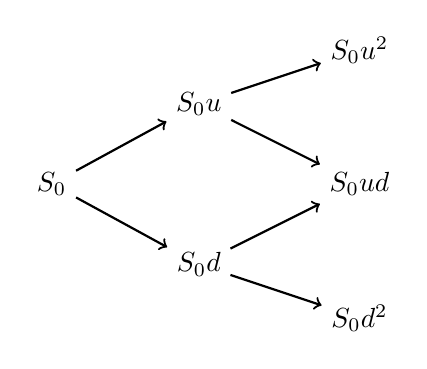
\begin{tikzpicture}[scale=0.85]
        \node (s0) at (0,0) {\(S_0\)};
        \node (su) at (2.2,1.2) {\(S_0u\)};
        \node (sd) at (2.2,-1.2) {\(S_0d\)};
        \node (suu) at (4.6,2.0) {\(S_0u^2\)};
        \node (sud) at (4.6,0) {\(S_0ud\)};
        \node (sdd) at (4.6,-2.0) {\(S_0d^2\)};
        \draw[->,thick] (s0) -- (su);
        \draw[->,thick] (s0) -- (sd);
        \draw[->,thick] (su) -- (suu);
        \draw[->,thick] (su) -- (sud);
        \draw[->,thick] (sd) -- (sud);
        \draw[->,thick] (sd) -- (sdd);
    \end{tikzpicture}
    \end{center}

    Recombining trees keep the number of nodes manageable.
\end{frame}

\begin{frame}{Backward Induction}
    \begin{enumerate}
        \item Compute terminal option payoffs.
        \item Step backward one period at a time.
        \item At each node, use
        \[
            f=e^{-r\Delta t}\left[p f_u+(1-p)f_d\right].
        \]
    \end{enumerate}

    \vspace{0.6em}
    For two steps:
    \[
        f_u=e^{-r\Delta t}\left[p f_{uu}+(1-p)f_{ud}\right],
    \]
    \[
        f_d=e^{-r\Delta t}\left[p f_{ud}+(1-p)f_{dd}\right],
    \]
    \[
        f=e^{-r\Delta t}\left[p f_u+(1-p)f_d\right].
    \]
\end{frame}

\begin{frame}{Two-Step European Put Example}
    \small
    Consider a two-year European put:
    \[
        S_0=50,\quad K=52,\quad u=1.2,\quad d=0.8,\quad r=5\%,\quad \Delta t=1.
    \]
    Risk-neutral probability:
    \[
        p=\frac{e^{0.05}-0.8}{1.2-0.8}\approx 0.6282.
    \]
    Terminal stock prices:
    \[
        72,\quad 48,\quad 32.
    \]
    Terminal put payoffs:
    \[
        f_{uu}=0,\quad f_{ud}=4,\quad f_{dd}=20.
    \]
    Price:
    \[
        f=e^{-0.10}
        \left[(0.6282)^2(0)+2(0.6282)(0.3718)(4)+(0.3718)^2(20)\right]
        \approx 4.19.
    \]
\end{frame}

\begin{frame}{American Option Trees}
    For American options, every node has an exercise decision.

    \begin{block}{Continuation value}
        \[
            e^{-r\Delta t}\left[p f_u+(1-p)f_d\right].
        \]
    \end{block}

    \begin{block}{American put node value}
        \[
            \max\left[
                K-S,\,
                e^{-r\Delta t}\left(p f_u+(1-p)f_d\right)
            \right].
        \]
    \end{block}

    \begin{alertblock}{Algorithm}
        Work backward. At each node, compute continuation value, compute exercise value, and keep the larger.
    \end{alertblock}
\end{frame}

\begin{frame}{American Put Node Example}
    At a node in an American put tree:
    \[
        S=38,\quad K=45,\quad r=4\%,\quad \Delta t=0.5,\quad p=0.55,
    \]
    \[
        f_u=5,\qquad f_d=12.
    \]

    Continuation value:
    \[
        e^{-0.04(0.5)}[0.55(5)+0.45(12)]
        =
        e^{-0.02}(8.15)
        \approx 7.99.
    \]

    Exercise value:
    \[
        K-S=45-38=7.
    \]

    Node value is \(7.99\), so the put is not exercised at this node.
\end{frame}

\begin{frame}{Choosing \(u\), \(d\), and \(p\)}
    A tree with time step \(\Delta t\) is matched to volatility by setting
    \[
        u=e^{\sigma\sqrt{\Delta t}},
        \qquad
        d=e^{-\sigma\sqrt{\Delta t}}=\frac{1}{u}.
    \]

    Once \(u\) and \(d\) are chosen, no-arbitrage fixes
    \[
        p=\frac{e^{r\Delta t}-d}{u-d}.
    \]

    \begin{alertblock}{Measure change intuition}
        Moving from the real-world measure to the risk-neutral measure changes expected returns, not the volatility used to build the tree.
    \end{alertblock}
\end{frame}

\begin{frame}{Tree Parameter Example}
    Suppose
    \[
        \sigma=30\%,
        \qquad
        r=5\%,
        \qquad
        \Delta t=1.
    \]
    Then
    \[
        u=e^{0.30}=1.3499,
        \qquad
        d=e^{-0.30}=0.7408.
    \]
    The risk-neutral probability is
    \[
        p=\frac{e^{0.05}-0.7408}{1.3499-0.7408}
        \approx 0.5097.
    \]

    These parameters define the tree. Valuation then proceeds by backward induction.
\end{frame}

\begin{frame}{Increasing the Number of Steps}
    If option life is \(T\) and there are \(n\) steps:
    \[
        \Delta t=\frac{T}{n}.
    \]

    Use
    \[
        u=e^{\sigma\sqrt{\Delta t}},
        \qquad
        d=e^{-\sigma\sqrt{\Delta t}},
        \qquad
        p=\frac{e^{r\Delta t}-d}{u-d}.
    \]

    \begin{block}{Convergence}
        As \(n\) increases, the time grid becomes finer.
        For European options on non-dividend-paying stocks, the binomial price converges to the Black-Scholes-Merton price.
    \end{block}
\end{frame}

\begin{frame}{Five-Step Illustration}
    Suppose
    \[
        T=2,\quad n=5,\quad r=5\%,\quad \sigma=30\%.
    \]
    Then
    \[
        \Delta t=\frac{2}{5}=0.4.
    \]

    \[
        u=e^{0.30\sqrt{0.4}}\approx 1.2089,
        \qquad
        d=\frac{1}{u}\approx 0.8272.
    \]

    \[
        e^{r\Delta t}=e^{0.05(0.4)}\approx 1.0202,
    \]

    \[
        p=\frac{1.0202-0.8272}{1.2089-0.8272}\approx 0.5056.
    \]
\end{frame}

\section{Review}

\begin{frame}{What We Omitted}
    \begin{block}{Intentional exclusions}
        The source material includes:
        \begin{itemize}
            \item Section 13.10 on DerivaGem software;
            \item Section 13.11 on options on other assets.
        \end{itemize}
    \end{block}

    \vspace{0.5em}
    These slides follow the lecture notes and exclude those sections.
    The binomial-tree discussion here is limited to stock options through increasing the number of steps.
\end{frame}

\begin{frame}{Checklist}
    After this lecture you should be able to:
    \begin{itemize}
        \item compute payoffs and profits for long and short calls and puts;
        \item interpret moneyness, intrinsic value, and time value;
        \item explain why option writers post margin;
        \item list the inputs that affect call and put prices;
        \item derive option upper and lower bounds;
        \item use put-call parity and identify parity arbitrage;
        \item explain early exercise for American calls and puts;
        \item price one-step and two-step binomial trees;
        \item compute delta and interpret the hedge;
        \item choose \(u\), \(d\), and \(p\) from volatility and the time step.
    \end{itemize}
\end{frame}

\begin{frame}{Practice Problems}
    \small
    \begin{enumerate}
        \item A call has strike 60 and premium 4. Compute payoff and profit for \(S_T=52,60,71\).
        \item A put has strike 45 and premium 3.50. Compute payoff and profit for \(S_T=35,45,52\).
        \item A European call costs 6.20. The stock is 50, the strike is 52, \(r=5\%\), and \(T=0.75\). Use put-call parity to compute the put price.
        \item A stock is 30 and can move to 36 or 24 in one year. A one-year call has strike 32 and \(r=5\%\). Compute \(p\), the call price, and delta.
        \item At an American put node, \(S=42\), \(K=50\), \(r=6\%\), \(\Delta t=0.25\), \(p=0.52\), \(f_u=5\), and \(f_d=11\). Should the option be exercised?
    \end{enumerate}
\end{frame}

\begin{frame}[plain,noframenumbering]
    \vfill
    \begin{center}
        {\usebeamerfont{title}\usebeamercolor[fg]{titlelike}Next Lecture\par}
        \vspace{0.8em}
        {\usebeamerfont{subtitle}Option trading strategies and payoff engineering\par}
    \end{center}
    \vfill
\end{frame}

\end{document}
